% !TEX root = rapport.tex

\section{Special-Purpose Devices}

Computers today are used for the most diverse set of tasks. They have become such an integral part of our society that people with handicaps that prevent them from using computers are at risk of getting left out of large parts of society and from work opportunities. While the computers themselves are indifferent towards handicaps, the input and output devices may present the user with accessibility problems.

The obstacles for people with impaired vision are mostly concerned with output devices, since most output devices rely on graphics like bitmap-displays or status LEDs. This can be circumvented with accessibility tools, such as the Apple \emph{VoiceOver} solution described below. But input methods may also present problems, for example the touchpads used in modern mobile phones.

For people with reduced motor skills, the obstacles lie mainly in the use of input devices and come in many different degrees. The standard computer mouse can be too sensitive for some users, while for other users both the mouse and keyboard may be unusable. Below, some of the most prominently used special-purpose devices are described.

Devices aimed towards aiding people with reduced motor skills come in different types, depending on which problem they are designed to solve. In some cases the use of hand-controlled devices is an issue, which has led to research on alternative keyboard solutions. In 1997 \cite{583209} a foot-controlled keyboard was described for persons having atleast one foot. It consists of an arched set of keys centered around the heel of the foot, used for typing. This kind of input device is aimed at amputees and persons with cerebral palsy. This demonstrates the specific nature of some existing solutions. Other methods are designed to be more general, allowing usage of persons with several types of disabilities, such as gaze communication, see below. 

A set of devices currently in research are devices controlled using eyes or facial features which do not require any other movement. These devices are called \emph{gaze communication devices}. Devices that use gaze communication are often designed to allow persons who have extensive motor skill handicaps to rely on facial features and actions for controlling the cursor on the display, like nose tip and pupil movements for cursor movements and blinking for performing click actions\cite{ieee6398171}\cite{conf/itng/AraiM11a}.

Since computer output is mainly dependent on displays, the implementation of special computer interfaces for blind or vision impaired persons is needed. One such solution has been the introduction of tactile braille displays. These displays consist of a bit matrix, where each bit can be raised or lowered to generate braille text. This creates a computer interaction interface that removes the barrier of vision from computer use. Previously these systems have been adapted for command line interfaces, in the last few years however, there has been research on Braille Window Systems, enabling interaction with graphical user interfaces through tactile displays\cite{prescher2010tactile}\cite{conf/petra/SturmSKJ09}. These interfaces work in a way similar to touchscreen devices, in that they move the control of the user interface from a separate input device to the output device. Tests show that users find these systems efficient, however, they require some time to get accustomed to.

\begin{figure}[h!]
\missingfigure{Braille display. Waiting for permission.}
%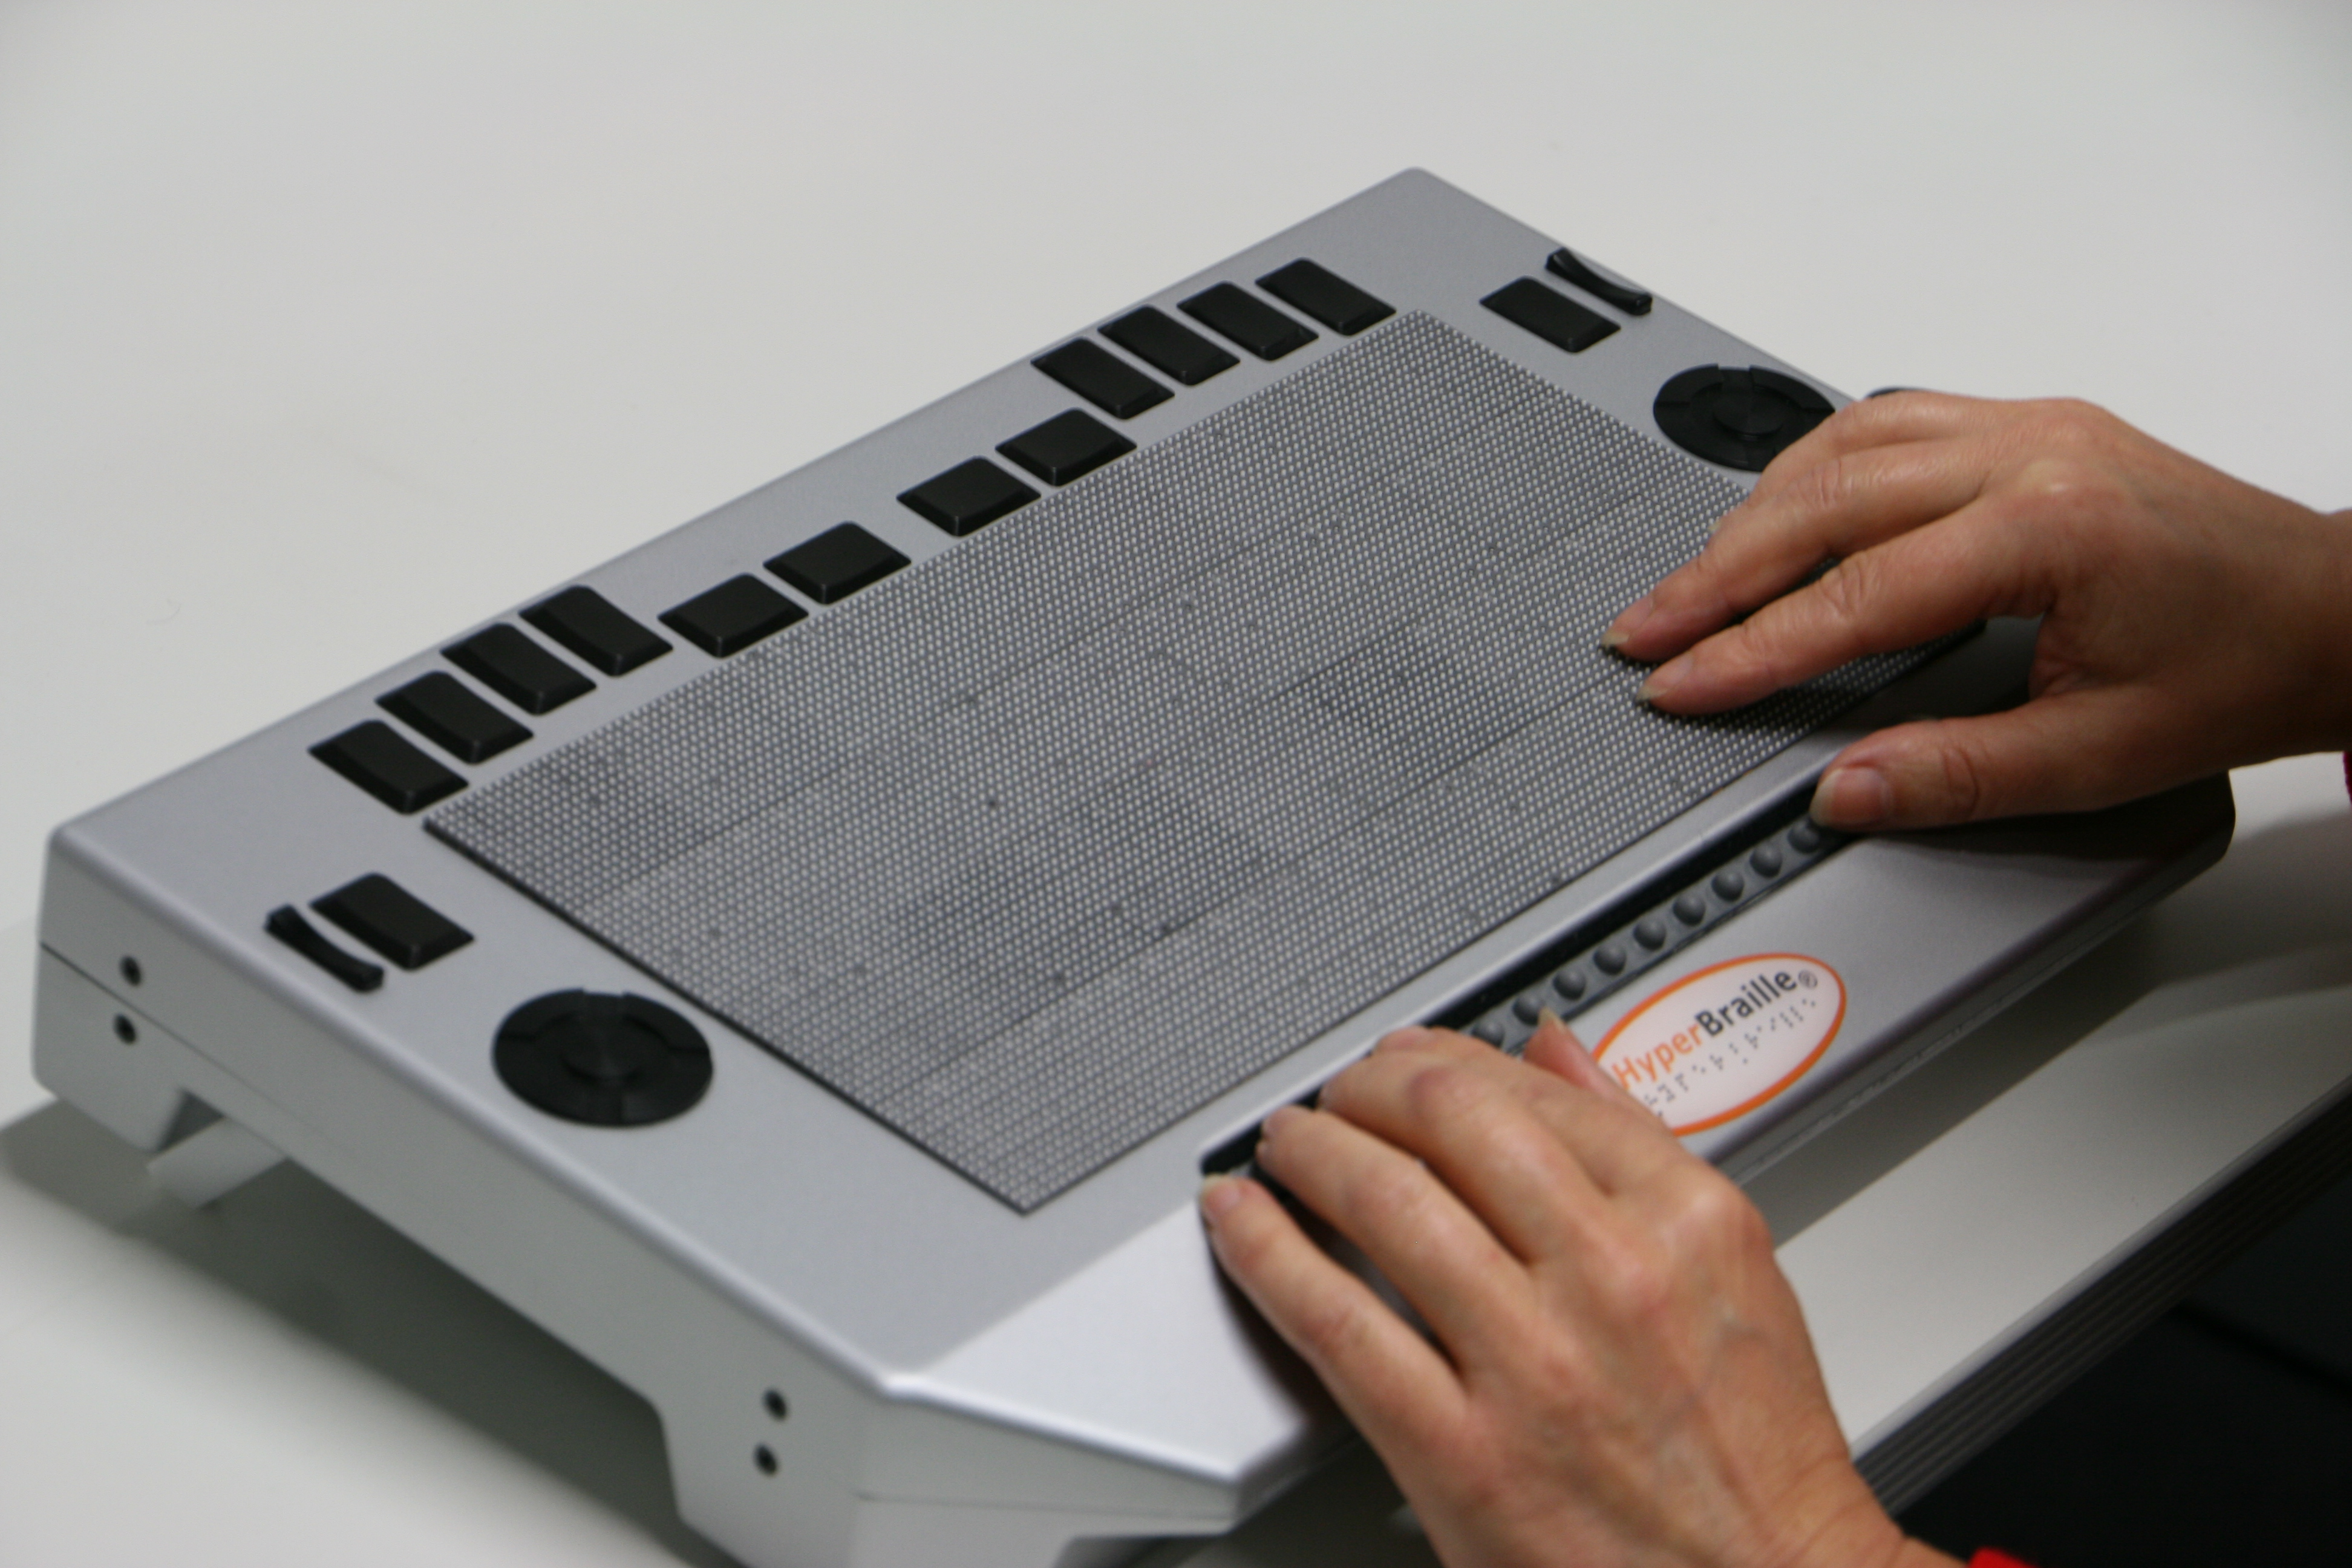
\includegraphics[width=0.8\textwidth] {bilder/IMG_7722.JPG}
\caption{A tactical braille display.}
\label{brailledisplay}
\end{figure}
\nocite{brailledisplay}


Advances in regular interaction technology can also contribute to the development of special-purpose devices. An example thereof is the Perkinput method\cite{azenkot}. The method allows the user to enter text in a much faster pace when handling touchscreen devices in comparison to text-to-speech methods, used in VoiceOver and other similar solutions. The method allows the user to enter \emph{Braille}\footnote{Writing system used by the blind.} letters directly by tapping fingers on the display.

The Braille alphabet is built using a 2x3 \emph{bit\footnote{The elevations used in Braille letters are known as bits, but differ from the bits used in computer systems.} matrix} where each letter has certain \emph{bits} "up" or "down", see figure \ref{fig:brailleexample}. In the Perkinput system, using two hand Braille input the user taps up to six fingers on the display - each finger representing a bit in the Braille letters. The letters can also be entered using only one hand by first entering the left column with three fingers, followed by the right column with the same fingers.

\begin{figure}[h!]
\centering

\begin{tabular}{c c c}

$
\begin{array}{cc}
\bullet & \circ \\
\bullet & \circ \\
\circ & \circ \end{array}
$

&

$
\left[ \begin{array}{cc}
1 & 0 \\
1 & 0 \\
0 & 0 \end{array} \right]
$ 

&

110000 \\

(a) & (b) & (c)

\end{tabular}


\caption{Three representations of the Braille letter B; the regular representation (a), a matrix representation (b), and a binary representation (c).}
\label{fig:brailleexample}


\end{figure}


For entering letters using two hands, the user uses three fingers on each hand. Each finger represents one of the bits in the Braille letter. To enter the letter B, having binary representation 110000 using two hands, the user would press the first two fingers on the first hand only, representing only the first two bits as 1:s.

To enter the letter B, using one hand, the user would press the two first fingers to represent 110, and then do a one finger swipe to represent the remaining 000.

The input rate of this special-purpose method is evidentially faster than the iPhones standard input method\cite{azenkot}, and two handed Perkinput is more than twice as fast. This comparison shows the difference a special-purpose device can make in the effectiveness of computer use related to adapted standard input methods. 

